\documentclass[14pt]{extbook}
\usepackage{multicol, enumerate, enumitem, hyperref, color, soul, setspace, parskip, fancyhdr} %General Packages
\usepackage{amssymb, amsthm, amsmath, bbm, latexsym, units, mathtools} %Math Packages
\everymath{\displaystyle} %All math in Display Style
% Packages with additional options
\usepackage[headsep=0.5cm,headheight=12pt, left=1 in,right= 1 in,top= 1 in,bottom= 1 in]{geometry}
\usepackage[usenames,dvipsnames]{xcolor}
\usepackage{dashrule}  % Package to use the command below to create lines between items
\newcommand{\litem}[1]{\item#1\hspace*{-1cm}\rule{\textwidth}{0.4pt}}
\pagestyle{fancy}
\lhead{Progress Quiz 1}
\chead{}
\rhead{Version C}
\lfoot{2654-6976}
\cfoot{}
\rfoot{Fall 2020}
\begin{document}

\begin{enumerate}
\litem{
First, find the equation of the line containing the two points below. Then, write the equation as $ y=mx+b $ and choose the intervals that contain $m$ and $b$.\[ (5, 3) \text{ and } (-7, -6) \]\begin{enumerate}[label=\Alph*.]
\item \( m \in [0.75, 2.75] \hspace*{3mm} b \in [-0.91, -0.64] \)
\item \( m \in [0.75, 2.75] \hspace*{3mm} b \in [0.87, 1.29] \)
\item \( m \in [0.75, 2.75] \hspace*{3mm} b \in [-2.15, -1.76] \)
\item \( m \in [0.75, 2.75] \hspace*{3mm} b \in [0.75, 0.9] \)
\item \( m \in [-7.75, 0.25] \hspace*{3mm} b \in [-11.51, -11.22] \)

\end{enumerate} }
\litem{
Find the equation of the line described below. Write the linear equation as $ y=mx+b $ and choose the intervals that contain $m$ and $b$.\[ \text{Perpendicular to } 5 x - 7 y = 13 \text{ and passing through the point } (-9, 5). \]\begin{enumerate}[label=\Alph*.]
\item \( m \in [-3.1, -0.9] \hspace*{3mm} b \in [5.6, 11.6] \)
\item \( m \in [-3.1, -0.9] \hspace*{3mm} b \in [12, 16] \)
\item \( m \in [-0.2, 1.7] \hspace*{3mm} b \in [14.6, 19.6] \)
\item \( m \in [-1.1, 1.3] \hspace*{3mm} b \in [-11.6, -3.6] \)
\item \( m \in [-3.1, -0.9] \hspace*{3mm} b \in [-11.6, -3.6] \)

\end{enumerate} }
\litem{
Solve the equation below. Then, choose the interval that contains the solution.\[ -2(9x -8) = -4(6x -19) \]\begin{enumerate}[label=\Alph*.]
\item \( x \in [2.19, 4.19] \)
\item \( x \in [10, 13] \)
\item \( x \in [15.33, 19.33] \)
\item \( x \in [-16.33, -11.33] \)
\item \( \text{There are no real solutions.} \)

\end{enumerate} }
\litem{
Solve the linear equation below. Then, choose the interval that contains the solution.\[ \frac{-4x + 3}{5} - \frac{-4x + 9}{7} = \frac{-9x + 8}{8} \]\begin{enumerate}[label=\Alph*.]
\item \( x \in [15, 16.5] \)
\item \( x \in [1.7, 4.2] \)
\item \( x \in [-1.2, -0.7] \)
\item \( x \in [0.1, 1] \)
\item \( \text{There are no real solutions.} \)

\end{enumerate} }
\litem{
Write the equation of the line in the graph below in Standard form $Ax+By=C$. Then, choose the intervals that contain $A, B, \text{ and } C$.
\begin{center}
    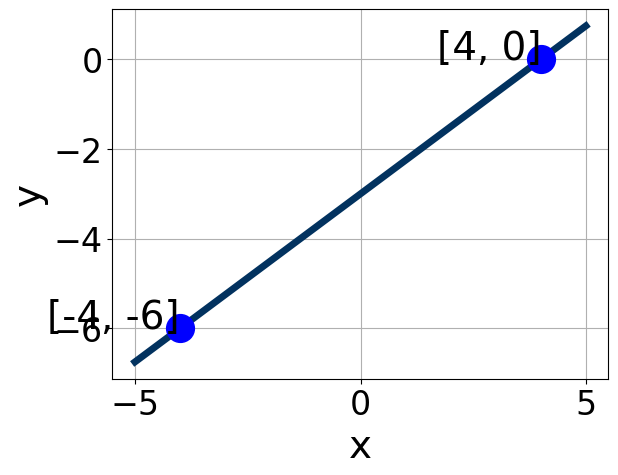
\includegraphics[width=0.5\textwidth]{../Figures/linearGraphToStandardCopyC.png}
\end{center}
\begin{enumerate}[label=\Alph*.]
\item \( A \in [-1.25, 3.75], \hspace{3mm} B \in [-2, 0.6], \text{ and } \hspace{3mm} C \in [4, 6] \)
\item \( A \in [-1.25, 3.75], \hspace{3mm} B \in [0.7, 2.3], \text{ and } \hspace{3mm} C \in [-11, -3] \)
\item \( A \in [-7, -3], \hspace{3mm} B \in [2.3, 5.8], \text{ and } \hspace{3mm} C \in [-25, -15] \)
\item \( A \in [1, 12], \hspace{3mm} B \in [-5.3, -3.2], \text{ and } \hspace{3mm} C \in [17, 22] \)
\item \( A \in [1, 12], \hspace{3mm} B \in [2.3, 5.8], \text{ and } \hspace{3mm} C \in [-25, -15] \)

\end{enumerate} }
\litem{
Solve the linear equation below. Then, choose the interval that contains the solution.\[ \frac{-7x -6}{6} - \frac{-3x + 6}{5} = \frac{-7x -3}{8} \]\begin{enumerate}[label=\Alph*.]
\item \( x \in [-0.39, 2.61] \)
\item \( x \in [4.92, 7.92] \)
\item \( x \in [-2.86, 0.14] \)
\item \( x \in [25.19, 32.19] \)
\item \( \text{There are no real solutions.} \)

\end{enumerate} }
\litem{
Write the equation of the line in the graph below in Standard form $Ax+By=C$. Then, choose the intervals that contain $A, B, \text{ and } C$.
\begin{center}
    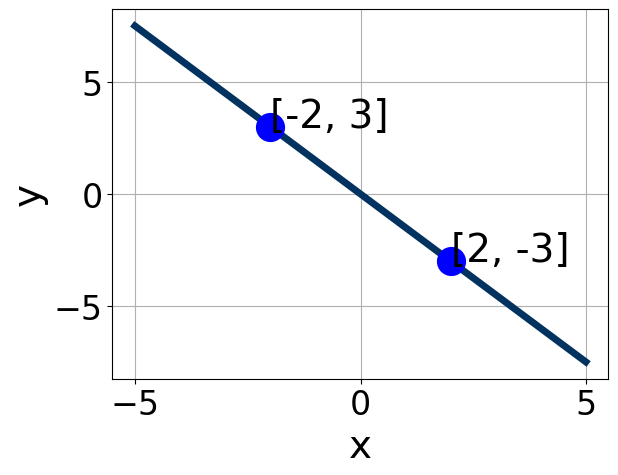
\includegraphics[width=0.5\textwidth]{../Figures/linearGraphToStandardC.png}
\end{center}
\begin{enumerate}[label=\Alph*.]
\item \( A \in [3.6, 5.3], \hspace{3mm} B \in [2.7, 3.3], \text{ and } \hspace{3mm} C \in [-11, -8] \)
\item \( A \in [-0.4, 2], \hspace{3mm} B \in [-2.7, 0.8], \text{ and } \hspace{3mm} C \in [0, 4] \)
\item \( A \in [-0.4, 2], \hspace{3mm} B \in [0.6, 2.9], \text{ and } \hspace{3mm} C \in [-5, -2] \)
\item \( A \in [-6.4, -0.9], \hspace{3mm} B \in [-5.8, -1.5], \text{ and } \hspace{3mm} C \in [5, 10] \)
\item \( A \in [3.6, 5.3], \hspace{3mm} B \in [-5.8, -1.5], \text{ and } \hspace{3mm} C \in [5, 10] \)

\end{enumerate} }
\litem{
First, find the equation of the line containing the two points below. Then, write the equation as $ y=mx+b $ and choose the intervals that contain $m$ and $b$.\[ (6, 3) \text{ and } (4, 4) \]\begin{enumerate}[label=\Alph*.]
\item \( m \in [-0.96, -0.03] \hspace*{3mm} b \in [5.86, 6.08] \)
\item \( m \in [-0.96, -0.03] \hspace*{3mm} b \in [-3.05, -1.99] \)
\item \( m \in [-0.96, -0.03] \hspace*{3mm} b \in [-6.62, -5.33] \)
\item \( m \in [-0.96, -0.03] \hspace*{3mm} b \in [-0.54, 0.67] \)
\item \( m \in [0.21, 0.96] \hspace*{3mm} b \in [1.63, 3.19] \)

\end{enumerate} }
\litem{
Solve the equation below. Then, choose the interval that contains the solution.\[ -16(-19x -18) = -5(13x -11) \]\begin{enumerate}[label=\Alph*.]
\item \( x \in [-0.81, -0.47] \)
\item \( x \in [0.77, 1.1] \)
\item \( x \in [-1.94, -1.29] \)
\item \( x \in [-0.94, -0.92] \)
\item \( \text{There are no real solutions.} \)

\end{enumerate} }
\litem{
Find the equation of the line described below. Write the linear equation as $ y=mx+b $ and choose the intervals that contain $m$ and $b$.\[ \text{Parallel to } 3 x + 5 y = 12 \text{ and passing through the point } (-10, 6). \]\begin{enumerate}[label=\Alph*.]
\item \( m \in [-1.31, 0.07] \hspace*{3mm} b \in [-1, 2] \)
\item \( m \in [-1.31, 0.07] \hspace*{3mm} b \in [13, 21] \)
\item \( m \in [0.21, 1.16] \hspace*{3mm} b \in [11, 14] \)
\item \( m \in [-1.31, 0.07] \hspace*{3mm} b \in [-1, 2] \)
\item \( m \in [-1.72, -1.59] \hspace*{3mm} b \in [-1, 2] \)

\end{enumerate} }
\end{enumerate}

\end{document}